\documentclass[12pt,a4paper]{article}
\usepackage[utf8]{inputenc}
\usepackage{amsmath}
\usepackage[]{units}
\usepackage{breqn}
\usepackage{amsfonts}
\usepackage{amssymb}
\usepackage{graphicx}
\usepackage[margin=0.8in]{geometry}


\begin{document}
\title{\vspace{70mm}\Huge Experimento 02 - Pêndulo de Torção}
\author{ Giovani Garuffi\qquad\hfill
		\textit {RA: 155559}\protect\\
		João Baraldi\hfill
		\textit{RA: 158044}\protect\\
		Lauro Cruz\hfill
		\textit{RA: 156175}\protect\\
		Lucas Schanner\hfill
		\textit{RA: 156412}\protect\\
		Pedro Stringhini\hfill
		\textit {RA: 156983}								
		}
\maketitle
\newpage
\section{Resumo}


\section{Objetivos}


\section{Procedimento Experimental e Coleta de Dados}

\subsection{Materiais utilizados}
\begin{itemize}
	\item Pêndulo de torção com fio metálico
	\item Trena
	\item Paquímetro
	\item Micrômetro
	\item Photo-gate
	\item Cronômetro inteligente
\end{itemize}

\subsection{Procedimento}
O pêndulo foi montado usando-se um fio metálico tendo um cilindro de latão acoplado em sua ponta. Foram medidos o diâmetro do fio (com o micrômetro) e contabilizada a massa do cilindro (já previamente neles explicitada). Ao lado do da base do pêndulo foi montado o photo-gate conectado a um cronômetro inteligente configurado no modo \emph{Pendulum} para ser realizada a medição dos perídos de rotação. Para cada comprimento L do fio foram feitas 7 medições de período para fazer-se assim um média aritmética. Todas as medições mencionadas estão presentes no relatório

\begin{figure}[!htbp]
	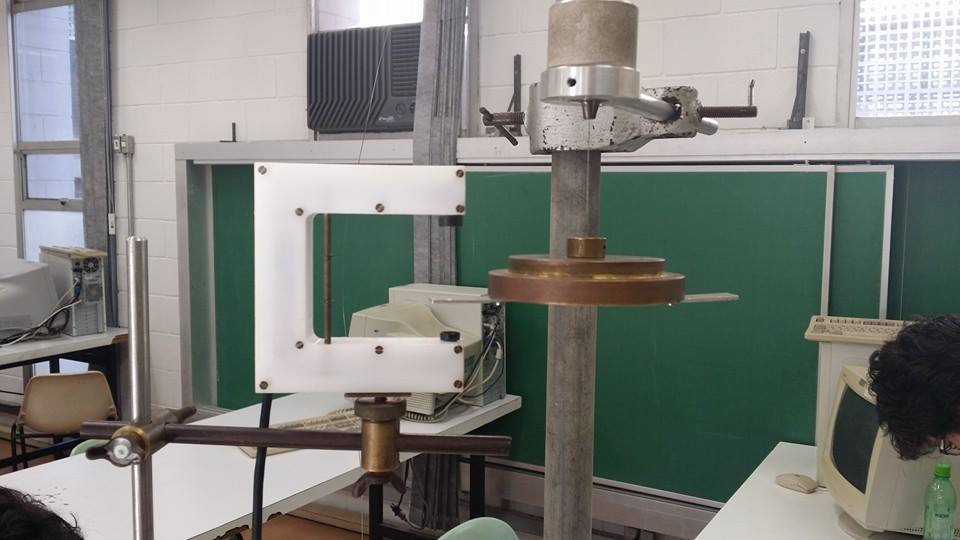
\includegraphics[scale=0.50]{03.jpg}
	\caption{Medição dos períodos}
	\label{fig:cilindro}
\end{figure}

\begin{figure}[!htbp]
	\centering
	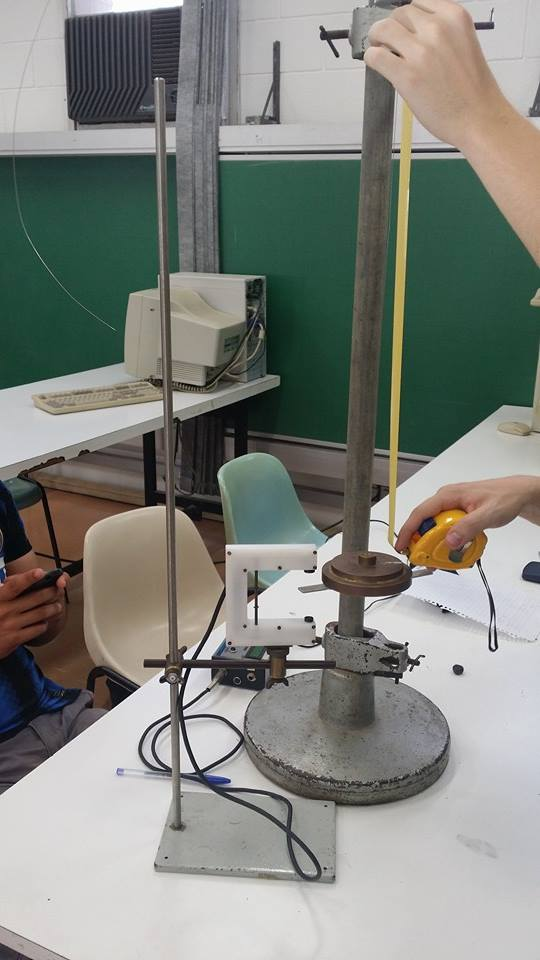
\includegraphics[scale=0.30]{01.jpg}
	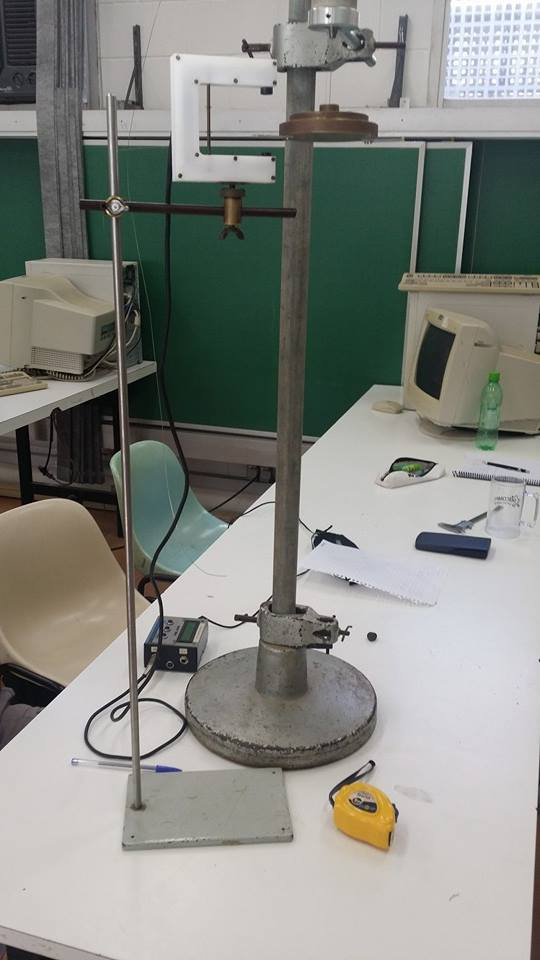
\includegraphics[scale=0.30]{02.jpg}\\
	Figures 1, 2: Montagem
\end{figure}

\subsection{Dados Obtidos}
O valor do diâmetro do fio é:
$$ d = (0.56 \pm 0.01) mm $$
Sendo $0.01 mm$ o erro intrumental do micrômetro.\\\\
Massa do conjunto de cilindros:
$$ m = (1198.2 \pm 0.1) g $$
Sendo $0.1 g$ o erro intrumental da balança usada.\\\\
Os valores dos períodos medidos (T) para cada comprimento da linha (L):

\subsubsection{Analise do cilindro}
Para fazer o cálculo do momento de inércia do cilindro utilizado no pêndulo ele foi subdividido em três cilindros (Figure \ref{fig:cilindro}), e foram medidos os diâmetros e alturas de cada um, para assim calcular seus volumes e determinar a massa de cada um separadamente.

Diâmetros:
$$ D_1 = (20.05 \pm 0.05)mm $$
$$ D_2 = (80.15 \pm 0.05)mm $$
$$ D_3 = (99.35 \pm 0.05)mm $$

Alturas:
$$ h_1 = (10.05 \pm 0.05)mm $$
$$ h_2 = (8.05 \pm 0.05)mm $$
$$ h_3 = (12.40 \pm 0.05)mm $$
Sendo $0.05mm$ o erro instrumental do paquímetro

\section{Análise dos Resultados e Discussões}


\section{Conclusões}


\end{document}
